\documentclass{beamer}
\usetheme{Madrid}
\usecolortheme{default}
\usepackage{listings}
\usepackage{tcolorbox}
\tcbuselibrary{listings, skins}

\newtcblisting{mycode}{
  arc=0mm,                          % Sharp corners
  boxrule=0.5pt,                    % Border thickness
  colback=white,                    % Background color
  colframe=black,                   % Border color
  listing only, 
  listing options={
    language=Python,
    basicstyle=\small\ttfamily,      % Monospace font
    keywordstyle=\color{blue},       % Color for 'import', etc.
    commentstyle=\color{blue},       % Color for comments
    stringstyle=\color{red},
    showstringspaces=false,
    breaklines=true
  },
  sharp corners,
  enhanced,
}
\usepackage{listings}
\usepackage{graphicx}

\lstset{
    language=Python,
    basicstyle=\ttfamily\small,
    keywordstyle=\bfseries,
    showstringspaces=false,
    breaklines=true
}

\title{Discrete-1.2.44}
\author{SAI HASINI PAPPULA-EE25BTECH11044}
\date{\today}

\begin{document}

\begin{frame}
\titlepage
\end{frame}

%--- Problem Statement ---
\begin{frame}{Problem}
\textbf{Solve the differential equation:}
\[
x\frac{dy}{dx} + y = x^4
\]
with boundary condition $y = 1$ at $x = 1$.

\vspace{1em}
\textbf{Options:}
\begin{enumerate}[(a)]
    \item $y = 5x^4 - 4$
    \item $y = x^4 + \dfrac{4x}{5}$
    \item $y = \dfrac{4x^4}{5} + \dfrac{1}{5x}$
    \item $y =\dfrac{x^4}{5} + \dfrac{4}{5x}$
\end{enumerate}
\end{frame}

%--- Step 1 ---
\begin{frame}{Step 1: Rewrite in Standard Form}
Divide throughout by $x$:
\[
\frac{dy}{dx} + \frac{1}{x}\,y = x^3
\]

This is the standard linear ODE form:
\[
\frac{dy}{dx} + P(x)\,y = Q(x)
\]
where
\[
P(x) = \frac{1}{x}, \qquad Q(x) = x^3
\]
\end{frame}

%--- Step 2 ---
\begin{frame}{Step 2: Integrating Factor}
The integrating factor is:
\[
\mu(x) = e^{\int P(x)\,dx} = e^{\int \frac{1}{x}\,dx} = e^{\ln x} = x
\]

Multiply both sides by $\mu(x) = x$:
\[
x\frac{dy}{dx} + y = x^4
\]

The left-hand side becomes a perfect derivative:
\[
\frac{d}{dx}\!\left(xy\right) = x^4
\]
\end{frame}

%--- Step 3 ---
\begin{frame}{Step 3: Integrate Both Sides}
\[
\frac{d}{dx}(xy) = x^4
\]

Integrating both sides with respect to $x$:
\[
xy = \frac{x^5}{5} + C
\]

Dividing by $x$:
\[
y = \frac{x^4}{5} + \frac{C}{x}
\]
\end{frame}

%--- Step 4 ---
\begin{frame}{Step 4: Apply Boundary Condition}
Apply $y = 1$ at $x = 1$:
\[
1 = \frac{1}{5} + \frac{C}{1} \implies C = 1 - \frac{1}{5} = \frac{4}{5}
\]

\vspace{0.5em}
\begin{block}{Final Solution}
\[
y = \frac{x^4}{5} + \frac{4}{5x}
\]
\end{block}
\end{frame}

%--- Verification ---
\begin{frame}{Verification}
\textbf{Check ODE:} $\quad y = \dfrac{x^4}{5} + \dfrac{4}{5x}$

\[
\frac{dy}{dx} = \frac{4x^3}{5} - \frac{4}{5x^2}
\]

\[
x\frac{dy}{dx} + y
  = \frac{4x^4}{5} - \frac{4}{5x} + \frac{x^4}{5} + \frac{4}{5x}
  = x^4 \checkmark
\]

\vspace{0.4em}
\textbf{Check BC:} $\quad y(1) = \dfrac{1}{5} + \dfrac{4}{5} = 1$ \checkmark

\vspace{0.6em}
\begin{block}{Conclusion}
\textbf{Option(d)  $\displaystyle y = \frac{x^4}{5} + \frac{4}{5x}$ is correct.}\\

\end{block}
\end{frame}

\begin{frame}[fragile]
\frametitle{Python Code for Plot}

\begin{mycode}
import numpy as np
import matplotlib.pyplot as plt

# Define x range (avoid x = 0)
x = np.linspace(0.1, 2, 1000)

# Solution of the differential equation
y = (x**4)/5 + 4/(5*x)

# Boundary condition
x_bc = 1
y_bc = 1

# Plot the solution
plt.figure()
plt.plot(x, y, label="y = x^4/5 + 4/(5x)")

\end{mycode}

\end{frame}

\begin{frame}[fragile]
\frametitle{Python Code for Plot}

\begin{mycode}

# Mark boundary condition
plt.scatter([x_bc], [y_bc])
plt.text(x_bc, y_bc, " (1,1)")

plt.title("Solution with Boundary Condition")
plt.xlabel("x")
plt.ylabel("y")
plt.grid()
plt.legend()
plt.show()
\end{mycode}

\end{frame}

\begin{frame}{Graph of the Solution}
\begin{center}
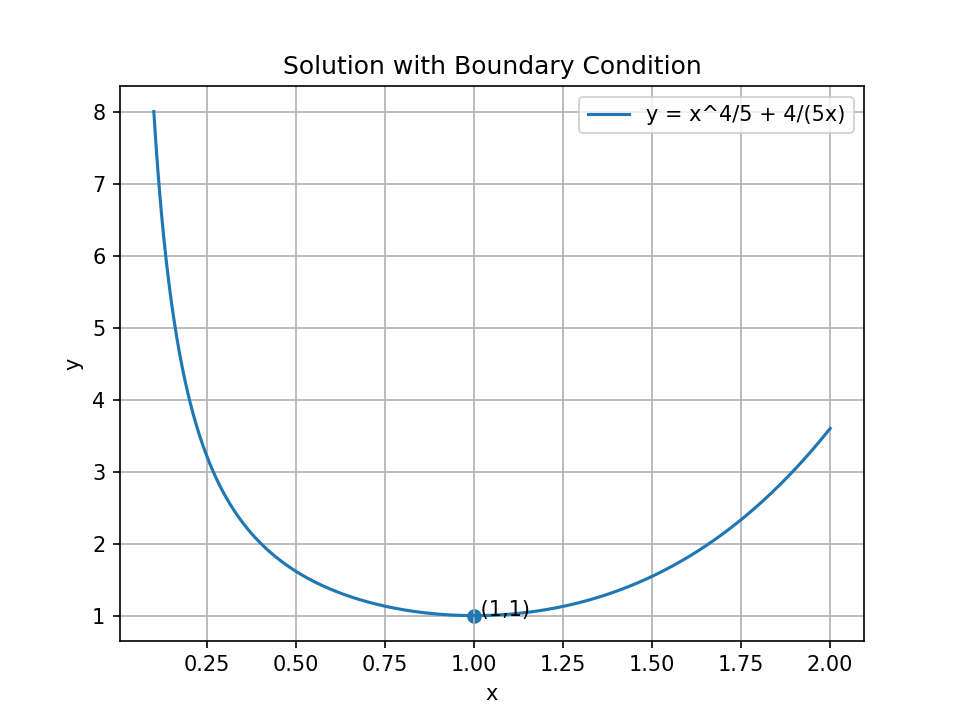
\includegraphics[width=0.8\textwidth]{plot2.png}
\end{center}

\begin{itemize}
\item Curve represents the solution
\item Point (1,1) satisfies boundary condition
\item Confirms correctness of solution
\end{itemize}
\end{frame}

\end{document}